%\documentstyle[epsf,twocolumn]{jarticle}       %LaTeX2.09仕様
\documentclass[twocolumn]{jarticle}     %pLaTeX2e仕様
%\documentclass[dvipdfmx,autodetect-engine]{ujarticle}	%???
%%%%%%%%%%%%%%%%%%%%%%%%%%%%%%%%%%%%%%%%%%%%%%%%%%%%%%%%%%%%%%
%%
%%  基本 バージョン
%%
%%%%%%%%%%%%%%%%%%%%%%%%%%%%%%%%%%%%%%%%%%%%%%%%%%%%%%%%%%%%%%%%
\setlength{\topmargin}{-45pt}
%\setlength{\oddsidemargin}{0cm}
\setlength{\oddsidemargin}{-7.5mm}
%\setlength{\evensidemargin}{0cm}
\setlength{\textheight}{24.1cm}
%setlength{\textheight}{25cm}
\setlength{\textwidth}{17.4cm}
%\setlength{\textwidth}{172mm}
\setlength{\columnsep}{11mm}

\kanjiskip=.07zw plus.5pt minus.5pt		%漢字と漢字の間に小さなグルーが入っている?その設定らしい


%【節がかわるごとに(1.1)(1.2) …(2.1)(2.2)と数式番号をつけるとき】tex
%\makeatletter
%\renewcommand{\theequation}{%
%\thesection.\arabic{equation}} %\@addtoreset{equation}{section}
%\makeatother

%\renewcommand{\arraystretch}{0.95} 行間の設定

%%%%%%%%%%%%%%%%%%%%%%%%%%%%%%%%%%%%%%%%%%%%%%%%%%%%%%%%
\usepackage[dvipdfm]{graphicx}   %pLaTeX2e仕様(要\documentstyle ->\documentclass)
\usepackage{url}
%%%%%%%%%%%%%%%%%%%%%%%%%%%%%%%%%%%%%%%%%%%%%%%%%%%%%%%%

\begin{document}

\twocolumn[		%全体を二段表示する場合には,一段表示したい部分を\twocolumn[]で囲めば良い
\noindent
\hspace{1em}

令和 5 年 1 月 24 日 (火) 情報工学実験 II 発表資料
\hfill
\ \ B3 味岡 陽紀

\vspace{2mm}
\hrule		%これはタイトルを囲む横線
\begin{center}
{\Large \bf Box Embedding による単語の分散表現獲得手法の検証}
\end{center}
\hrule
\vspace{3mm}
]

\section{はじめに}
深層学習など機械学習による自然言語処理は盛んな研究分野の一つである. 
自然言語処理はもちろん機械学習においても単語の表現や処理方法は文章の意味を計算によって解析するために必要不可欠な根幹的な要素である.
近年, Word2Vec のような単語のベクトル表現が広く使われる一方で単語の意味で表現することができない要素があることが認識されている. 
その代表的なものとして点でしかデータを表すことができないというものである. 
単語のベクトル埋め込みにおいてこのことは単語の意味の包含関係や階層関係といった集合的な性質を自然に表現できないということに起因する. 
このような問題を解決するための表現として領域表現が提案されており, ガウス分布を用いたものや双曲空間を用いたものがある. 
本実験では始点と終点の組で表される「箱」への単語埋め込み表現である Box Embedding を扱う. 

Box Embedding の獲得手法の一つとして Word2Box がある. 
この実験では Word2Box による単語埋め込み表現を獲得し, その埋め込み表現が単語間の意味をどのように表しているかを確認した. 

\section{要素技術}
\subsection{Box Embedding}
Box Embedding は d 次元のベクトルの組からなる「箱」の領域で単語を表現するものであり, Vilnis Luke ら\cite{box-lattice}によって提案された. 
図 \ref{fig:box_embedding2d} が示す mammal と carnivore の「箱」の共有部分にて cat の「箱」が存在するように, Box Embedding では「箱」同士の重なりによって単語の意味の包含関係や階層関係を表現する. 
しかし, Box Embedding は「箱」の重なりを調整することで表現を獲得するが, Vilnis Luke らによって提案された方法では「箱」が重ならないと勾配が計算できず最適化が難しくなる問題がある.
この問題に対して「箱」の境界を滑らかだとして領域を計算することで「箱」同士が離れていても勾配を求められ最適化できる. 
Sankar Dasgupta ら\cite{gumbel-box}によって提案された手法はそのうちの一つであり, Gumbel 分布を用いるものである. 
Gumbel 分布を適用した 2 次元での「箱」は図 \ref{fig:gumbel_box} のようになる. 

\begin{figure}[t]
  \centering
  \caption{2 次元での Box Embedding の例 (文献\cite{li2018smoothing} Figure 1 引用)}
  \label{fig:box_embedding2d}
  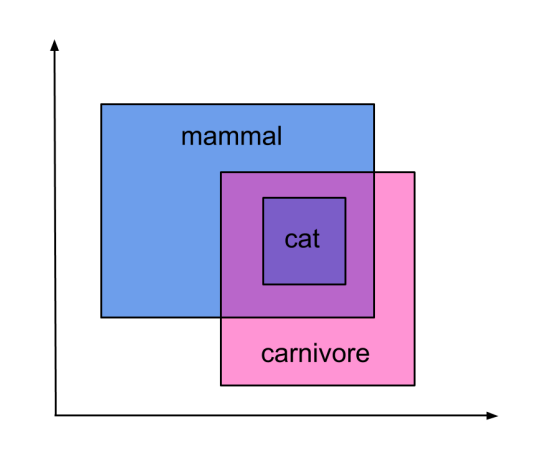
\includegraphics[width=70mm]{BoxEmbedding_2d.png}
\end{figure}

\begin{figure}[t]
  \centering
  \caption{2 次元での Gumbel Box の例 (文献\cite{pmlr-v161-boratko21a} Figure 3 引用)}
  \label{fig:gumbel_box}
  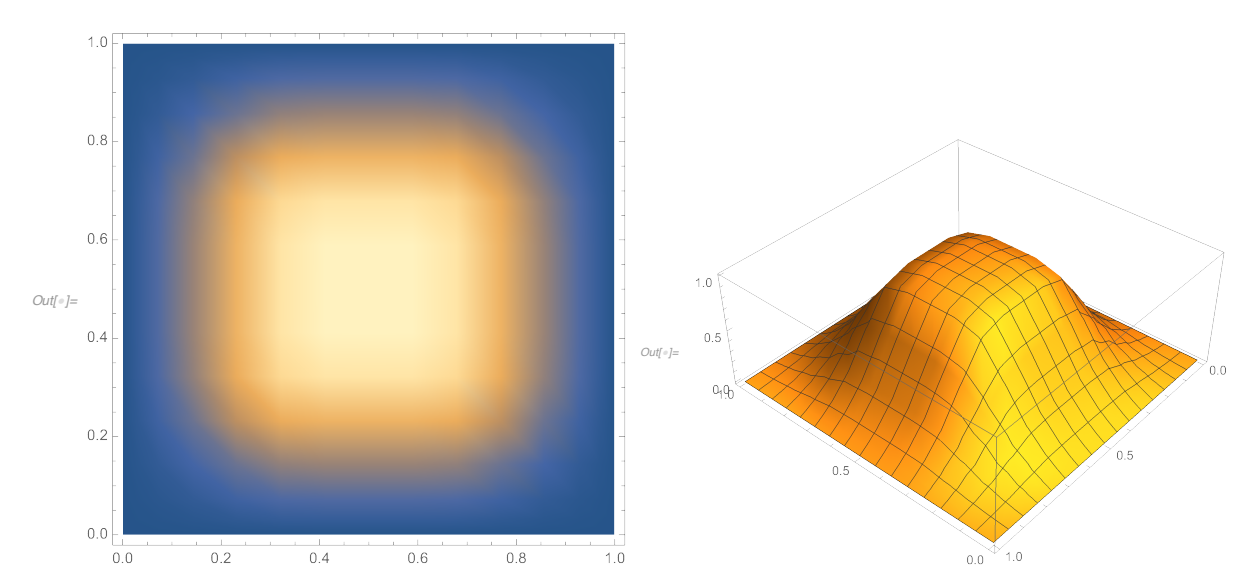
\includegraphics[width=70mm]{GumbelBoxes.png}
\end{figure}

\subsection{Word2Vec}
Word2Vec \cite{word2vec} は 2013 年に Google の Tomas Mikolov らによって発表された単語のベクトル埋め込み表現の生成モデルである. 
Word2Vec は 2 層ニューラルネットワークであり, 対象とする単語の周辺に現れる単語の頻度をもとに類似する周辺単語を持つ単語とのベクトルの類似度が大きくなるように学習する. 
周辺の単語から対象の単語を予測し学習する CBOW モデルと対象の単語から周辺の単語を予測し学習する Skip-gram モデルがある.

\subsection{Word2Box}
Word2Box \cite{dasgupta-etal-2022-word2box} は Sankar Dasgupta らによって提案された手法であり, 単語の領域表現の Box Embedding を教師なし学習で獲得するものである. 
学習方法は Word2Vec の CBOW モデルと同様に対象の単語とその周辺単語の「箱」の重なりが大きくなるように学習する. 
加えて, 「箱」をただ大きくする最適化にならないように適当な語を負例として抽出し周辺単語との重なりを小さくするように学習する. 

\section{データセット}
\subsection{Penn Treebank データセット}
Penn Treebank データセット\cite{ptb}は 	Mitchell P. Marcus らによって作成された 450 万語を超える大規模英語コーパスであり, コーパスには品詞情報も付加されている. 
この実験では数字を全て N , 語彙に含まれない単語を \textless unk\textgreater , パディングを \textless pad\textgreater としてそれぞれ一つの単語と見なして語彙数が 1 万語になるように調整されたものを用いた.

\subsection{単語類似度データセット}
\subsubsection{SimLex-999}
SimLex-999 \cite{simlex999} は Hill Felix らによって発表された英語の 999 組の単語間の関連性ではなく類似性に基づいて, 単語間の類似度を 0 から 10 の範囲で定量化したデータセットである. 

\subsubsection{WordSim-353}
WordSim-353 \cite{wordsim353} は Finkelstein Lev らによって作成された英語の 350 個の単語組をその関係度で 0 から 10 の範囲で評価したデータセットである.
このデータセットでは関連性と類似性による評価が混在しており, 関連する 252 単語組のサブセットである WS-353(Rel) と 類似する 203 単語組のサブセットである WS-353(Sim) がある.

\subsubsection{YP-130}
YP-130 は () らによって作成された英語の動詞の 130 個の単語組についての類似性を 0 から 4 の範囲で評価したデータセットである. 

\subsubsection{MEN}
MEN は () らによって作成された画像情報なども活用した英単語 3000 組についての意味的類似性

% \subsubsection{MC-30}

% \subsubsection{RG-65}

% \subsubsection{VERB-143}

% \subsubsection{Stanford RW}

% \subsubsection{Mturk-287}

% \subsubsection{Mturk-771}


\section{実験}
Word2Box の著者による実装 \url{https://github.com/iesl/word2box} を用いて表 \ref{tb:model_parameter} のパラメータで Penn Treebank コーパスから単語の埋め込みモデルを獲得をした. 
各単語類似度データセットをもとに類似度の高い単語の組について埋め込み表現同士での類似度を計算し, それぞれの単語においてもう一方の単語が類似度で学習した語彙の中で何番目に位置するかを求めた. 
各類似度データセットは数値の基準がそれぞれ異なるため, 表 \ref{tb:dataset_detail} に示す基準値を上回る単語組を実験に用いた. 
ただし, 基準値は各データセットの類似度の最大値の 80 \% としている. 
求めた結果から Word2Box が 2 単語間の類似性を適切に学習し Box Embedding で表現できているかを確認した. 

\begin{table}[th]
  \centering
  \caption{Word2Box モデルの学習パラメータ}
  \label{tb:model_parameter}
  \begin{tabular}{c|c} \hline
      parameter&value \\ \hline
      次元数&64 \\
      バッチサイズ&4096 \\ 
      エポック数&10 \\
      ウィンドウサイズ&5 \\
      ネガティブサンプル数&2 \\
      サブサンプル閾値&0.001 \\
      学習率&0.004204091643267762 \\
      \hline
  \end{tabular}
\end{table}

\begin{table*}[th]
  \centering
  \caption{類似度データセットから抽出した単語組}
  \label{tb:dataset_detail}
  \scalebox{0.6}[0.6]{
		\begin{tabular}{c|ccccccccccccc}
			\hline
			項目   & Stanford RW & RG-65 & YP-130 & MEN & MC-30 & Mturk-287 & SimVerb-3500 & SimLex-999 & Mturk-771 & WS-353(Sim) & WS-353(All) & WS-353(Rel) & VERB-143 \\ \hline
			基準値  & 8.0         & 3.2   & 3.2    & 40  & 3.2   & 4.0       & 3.2          & 8.0        & 4.0       & 8.0         & 8.0         & 8.0         & 3.2      \\
			該当組数 & 36          & 4     & 12     & 166 & 3     & 20        & 1053         & 68         & 85        & 16          & 31          & 14          & 0        \\ \hline
			\end{tabular}
  }
\end{table*}

\section{結果と考察}
実験結果は表 \ref{tb:result} のようになった. 
どのデータセットにおいても類似度が 1 から 99 番目に含まれる類似単語のペアはほとんど存在しなかった. 
それどころか上位 1000 番目までに含まれる類似単語ペアの割合は少数であった. 
また, 表 \ref{tb:rankdiff} のようにデータセットの種類にかかわらずほとんどの単語ペアにおいて類似度の順位を求める対象単語を入れ替えると順位が大きく変動することが確認された. 
ただし, ここで大きく変動したとする基準は順位が 1000 異なる場合とした. 
この大きく変動する組においても単語組が類似性を示す結果とはならなかった. 

次に類似度の順位が 1 から 99 番目に含まれていた単語組を表 \ref{tb:sim_words} に示す. 
含まれていた単語組と含まれなかった単語組との間に法則性を見出すことはできなかった. 


\begin{table}[th]
  \caption{類似単語ペアが含まれる順位}
  \label{tb:result}
  \begin{tabular}{c|ccc}
    \hline
    順位           & 1-99 & 100-499 & 500-999 \\ \hline
    Stanford RW  & 0    & 7       & 0       \\
    RG-65        & 0    & 0       & 0       \\
    YP-130       & 0    & 2       & 2       \\
    MEN          & 6    & 24      & 19      \\
    MC-30        & 0    & 0       & 0       \\
    Mturk-287    & 0    & 5       & 0       \\
    SimVerb-3500 & 19   & 74      & 86      \\
    SimLex-999   & 5    & 8       & 9       \\
    Mturk-771    & 1    & 11      & 3       \\
    WS-353(Sim)  & 1    & 1       & 2       \\
    WS-353(All)  & 2    & 1       & 2       \\
    WS-353(Rel)  & 1    & 0       & 0       \\
    VERB-143     & 0    & 0       & 0       \\ \hline
  \end{tabular}
\end{table}

\begin{table}[th]
  \centering
  \caption{対象単語入れ替えによる順位変動}
  \label{tb:rankdiff}
  \begin{tabular}{c|c|c}
    \hline
    データセット       & 変動が大きい組 & 組の総数 \\ \hline
    Stanford RW  & 28      & 36   \\
    RG-65        & 4       & 4    \\
    YP-130       & 9       & 12   \\
    MEN          & 123     & 166  \\
    MC-30        & 3       & 3    \\
    Mturk-287    & 14      & 20   \\
    SimVerb-3500 & 847     & 1053 \\
    SimLex-999   & 54      & 68   \\
    Mturk-771    & 53      & 85   \\
    WS-353(Sim)  & 14      & 16   \\
    WS-353(All)  & 24      & 31   \\
    WS-353(Rel)  & 10      & 14   \\
    VERB-143     & 0       & 0    \\ \hline
  \end{tabular}
\end{table}

\begin{table*}[th]
  \centering
  \caption{データセットごとのモデルによって類似度が高いとされた単語組}
  \label{tb:sim_words}
  \begin{tabular}{c|c}
    \hline
    データセット       & 類似単語組    \\ \hline
    MEN          & flight plane, highway traffic, cold frozen, mountain valley, bay beach, burger meat  \\ \hline
    SimVerb-3500 & \begin{tabular}[c]{@{}c@{}}let release, tell testify,release go, express tell, save rescue, release relax, tell predict,\\  spend use, say tell, tell respond, fight defend, rescue help, leave release, release drain,\\  release loosen, remove release, rescue find, gamble bet, gamble risk\end{tabular} \\ \hline
    SimLex-999   & essential necessary, area zone, pact agreement, physician doctor, expand grow  \\ \hline
    Mturk-771    & season winter \\ \hline
    WS-353(All)  & king queen, opec oil \\ \hline
    WS-353(Rel)  & opec oil    \\ \hline
    WS-353(Sim)  & king queen   \\ \hline
  \end{tabular}
\end{table*}

\section{今後の課題}
今回の実験結果は Word2Box によって獲得した Box Embedding について意味が近い単語間では似た分散表現になるという性質を示しておらず, その点において十分な表現能力があることを確認できなかった. 
提案論文において\cite{dasgupta-etal-2022-word2box}学習パラメータはいくつかの数値からランダムに選択することで決定し,実験とは異なる学習データを用いているため, 学習パラメータの調整や学習用の文章の変更によって性能の向上の可能性を模索する余地があると考えられる. 
また, Box Embedding の特徴の一つでもある集合による単語の意味の包含関係の表現や多義語に対する表現の検証を今回の実験ではできなかった. 

\bibliography{index}		%文献データベースindex.bibを使用する
\bibliographystyle{junsrt} 	%参考文献出力スタイル

\end{document}
